\chapter{Технологическая часть}

В данной части представляются выбор системы управления базами данных и средств реализации приложения, структуры приложения и базы данных, интерфейс приложения и тестирование.

\section{Выбор системы управления базами данных}

Наиболее распространёнными системами управления реляционными базами данных являются~\cite{lit11}:
\begin{itemize}[label=--]
	\item Oracle~\cite{lit12};
	\item MySQL~\cite{lit13};
	\item Microsoft SQL Server~\cite{lit14};
	\item PostgreSQL~\cite{lit15}.
\end{itemize}

Критерии сравнения систем управления реляционными базами данных представлены в таблице~\ref{tbl:subd-criteria}.

\begin{table}[h]
	\centering
	\caption{Критерии сравнения систем управления реляционными базами данных}
	\label{tbl:subd-criteria}
	\begin{tabularx}{\textwidth}{|p{3.5cm}|X|p{2.1cm}|}
		\hline
		\textbf{Критерий} & \textbf{Описание} & \textbf{Значения} \\
		\hline
		Бесплатная полная версия & Наличие полностью функциональной версии СУБД без ограничений, доступной для использования без оплаты лицензии & Да, нет \\
		\hline
		Возможность создавать роли, пользователей и управлять правами & Поддержка механизмов создания пользователей, ролей и тонкой настройки прав доступа к объектам БД на уровне SQL-запросов & Да, нет \\
		\hline
		Активная поддержка & Наличие официальной технической поддержки от разработчиков или активного сообщества, обеспечивающего регулярные обновления, исправления ошибок и документацию & Да, нет \\
		\hline
		Полное соответствие стандарту SQL & Строгое соблюдение стандартов SQL без использования расширений или отклонений от спецификаций & Да, нет \\
		\hline
	\end{tabularx}
\end{table}

\newpage

Результаты сравнительного анализа систем управления реляционными базами данных представлен в таблице~\ref{tbl:subd-compare}.

\begin{table}[h]
	\centering
	\caption{Сравнительный анализ систем управления реляционными базами данных}
	\label{tbl:subd-compare}
	\begin{tabularx}{\textwidth}{|p{3.5cm}|X|X|X|X|}
		\hline
		\textbf{Критерий} & \textbf{Oracle} & \textbf{MySQL} & \textbf{Microsoft SQL Server} & \textbf{PostgreSQL} \\
		\hline
		Бесплатная полная версия & Нет & Да & Нет & Да \\
		\hline
		Возможность создавать роли, пользователей и управлять правами & Да & Да & Да & Да \\
		\hline
		Активная поддержка & Да & Да & Да & Да \\
		\hline
		Полное соответствие стандарту SQL & Нет & Нет  & Нет & Да \\
		\hline
	\end{tabularx}
\end{table}

Для достижения поставленной цели была выбрана PostgreSQL благодаря её широкому набору инструментов, который отвечает всем необходимым критериям.

\section{Выбор средств реализации приложения}

В качестве языка программирования для реализации приложения был выбран $C\#$ по следующим причинам:
\begin{itemize}[label=--]
	\item поддержка объектно-ориентированной методологии программирования;
	\item присутствие в стандартной библиотеке языка необходимых типов данных, структур и классов, выбранных по результатам проектирования;
	\item возможность выполнения запросов к базе данных на уровне языка благодаря механизму LINQ~\cite{lit16}.
\end{itemize}

\section{Структуры приложения и базы данных}

Структура приложения соответствует спроектированной логике, отраженной на диаграммах~\ref{fig:data-flow},~\ref{fig:components-diagram} и~\ref{fig:class-diagram}.

Сопоставление типов данных к типам данных выбранной СУБД представлено в таблице~\ref{tbl:db-types}.

\begin{table}[h]
	\centering
	\caption{Сопоставление типов данных к типам выбранной СУБД}
	\label{tbl:db-types}
	\begin{tabularx}{\textwidth}{|X|X|}
		\hline
		\textbf{Тип данных} & \textbf{Тип данных СУБД} \\
		\hline
		Целочисленный & INT \\
		\hline
		Строковый & VARCHAR(255), TEXT \\
		\hline 
		Вещественный & NUMERIC(14,2) \\
		\hline
		Логический & BOOL \\
		\hline 
		Перечисляемый & ENUM \\
		\hline
		Дата & DATE \\
		\hline
	\end{tabularx}
\end{table}

Структура базы данных соответстует спроектированной логике, отраженной на диаграмме~\ref{fig:db-diagram}.

\begin{figure}[h!]
	\centering
	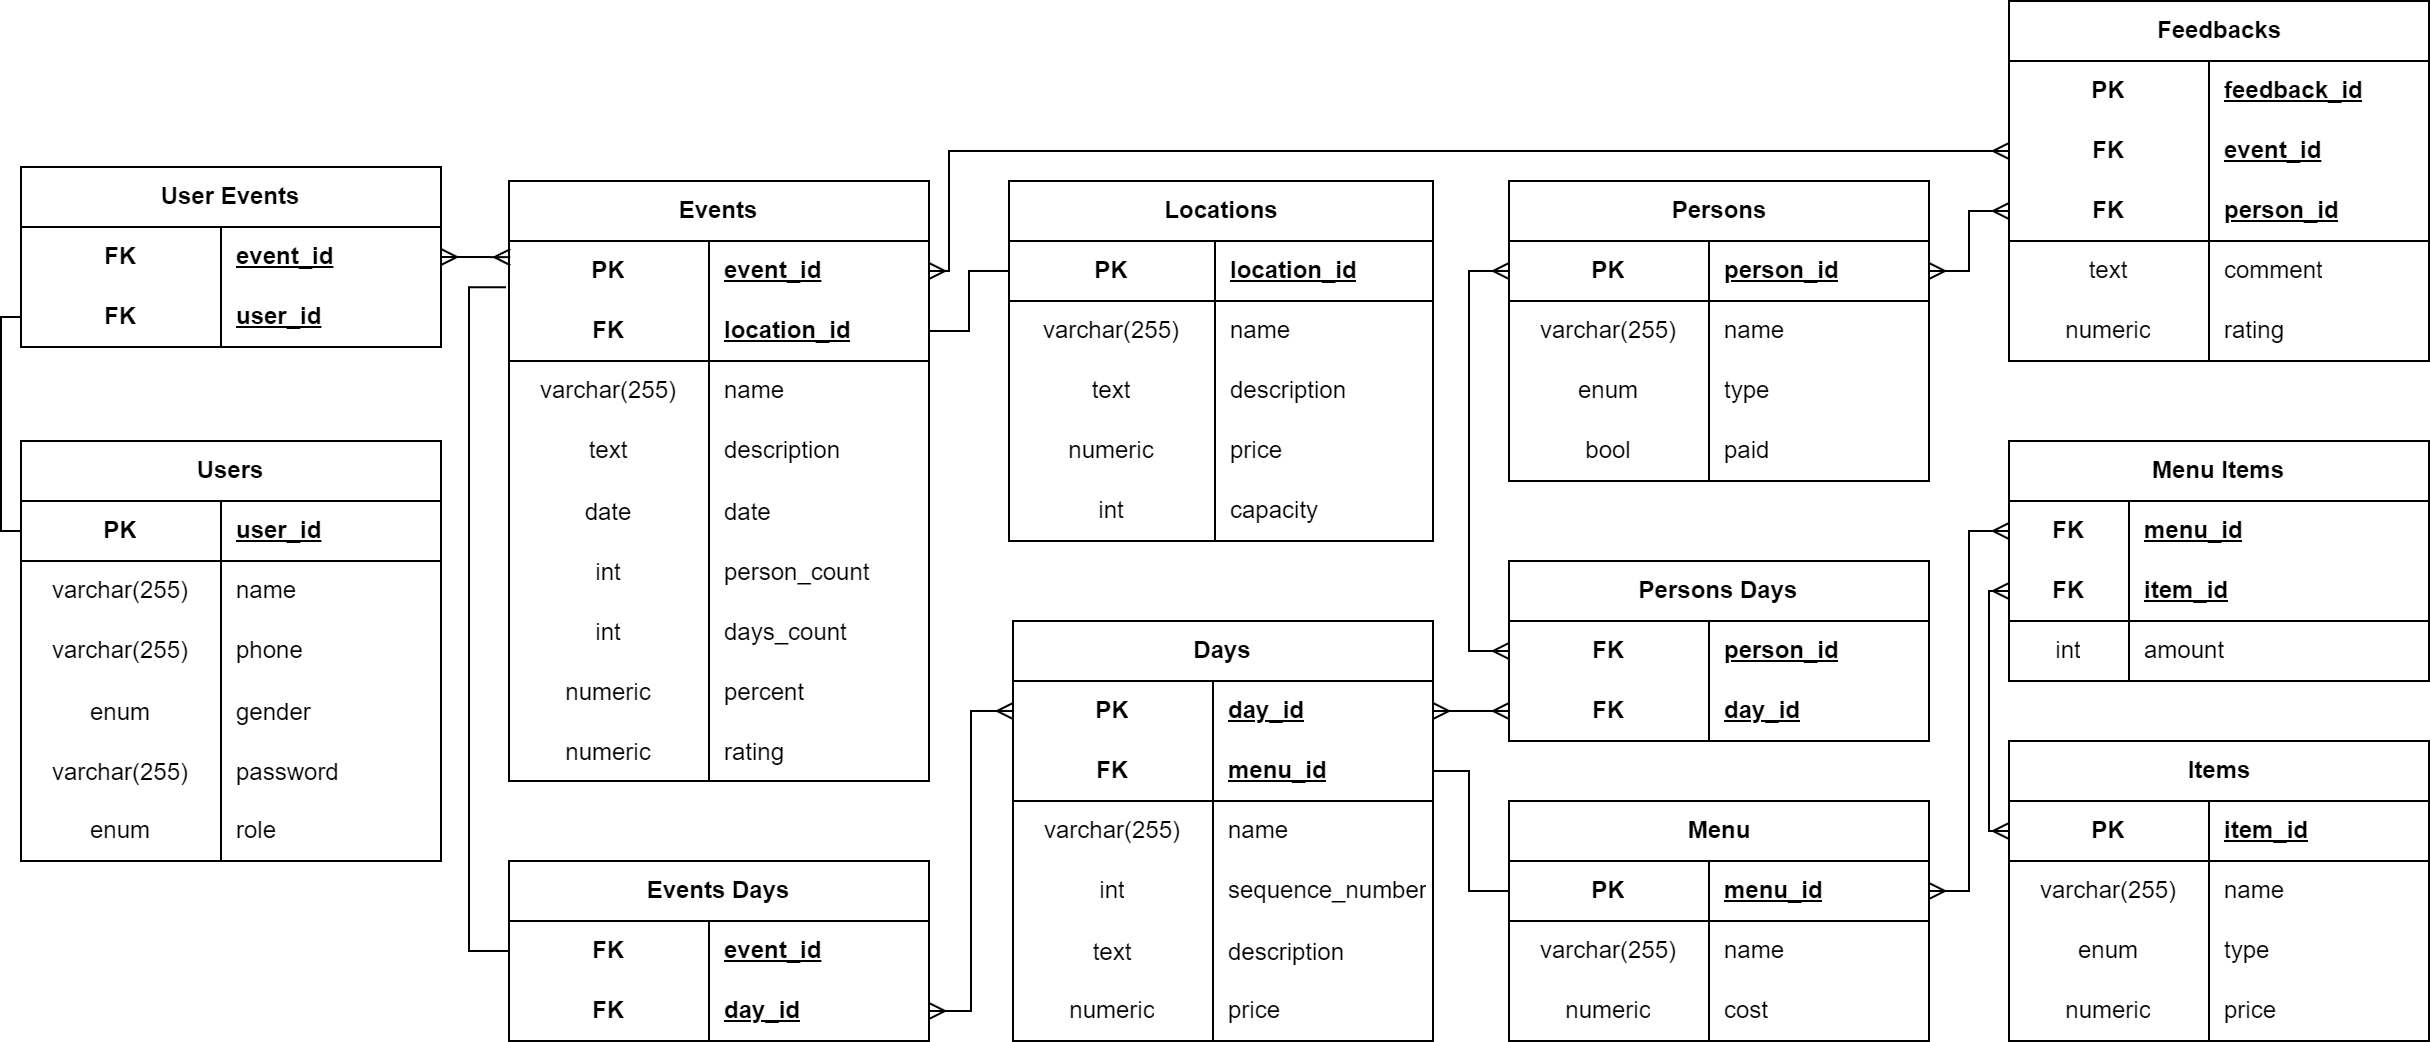
\includegraphics[width=1\textwidth]{images/db-diagram.png}
	\caption{Диаграмма базы данных (типы данных СУБД)} 
	\label{fig:db-diagram} 
\end{figure}

Исходный код реализованных приложения и базы данных доступен в открытом сетевом репозитории~\cite{lit17, lit18}.

\section{Интерфейс приложения}

При запуске приложения пользователю демонстрируется окно <<Вход в систему>>, предназначенную для регистрации и авторизации в системе. Текстовые поля обеспечивают возможность заполнить личные данные.

\newpage

\begin{figure}[h!]
	\centering
	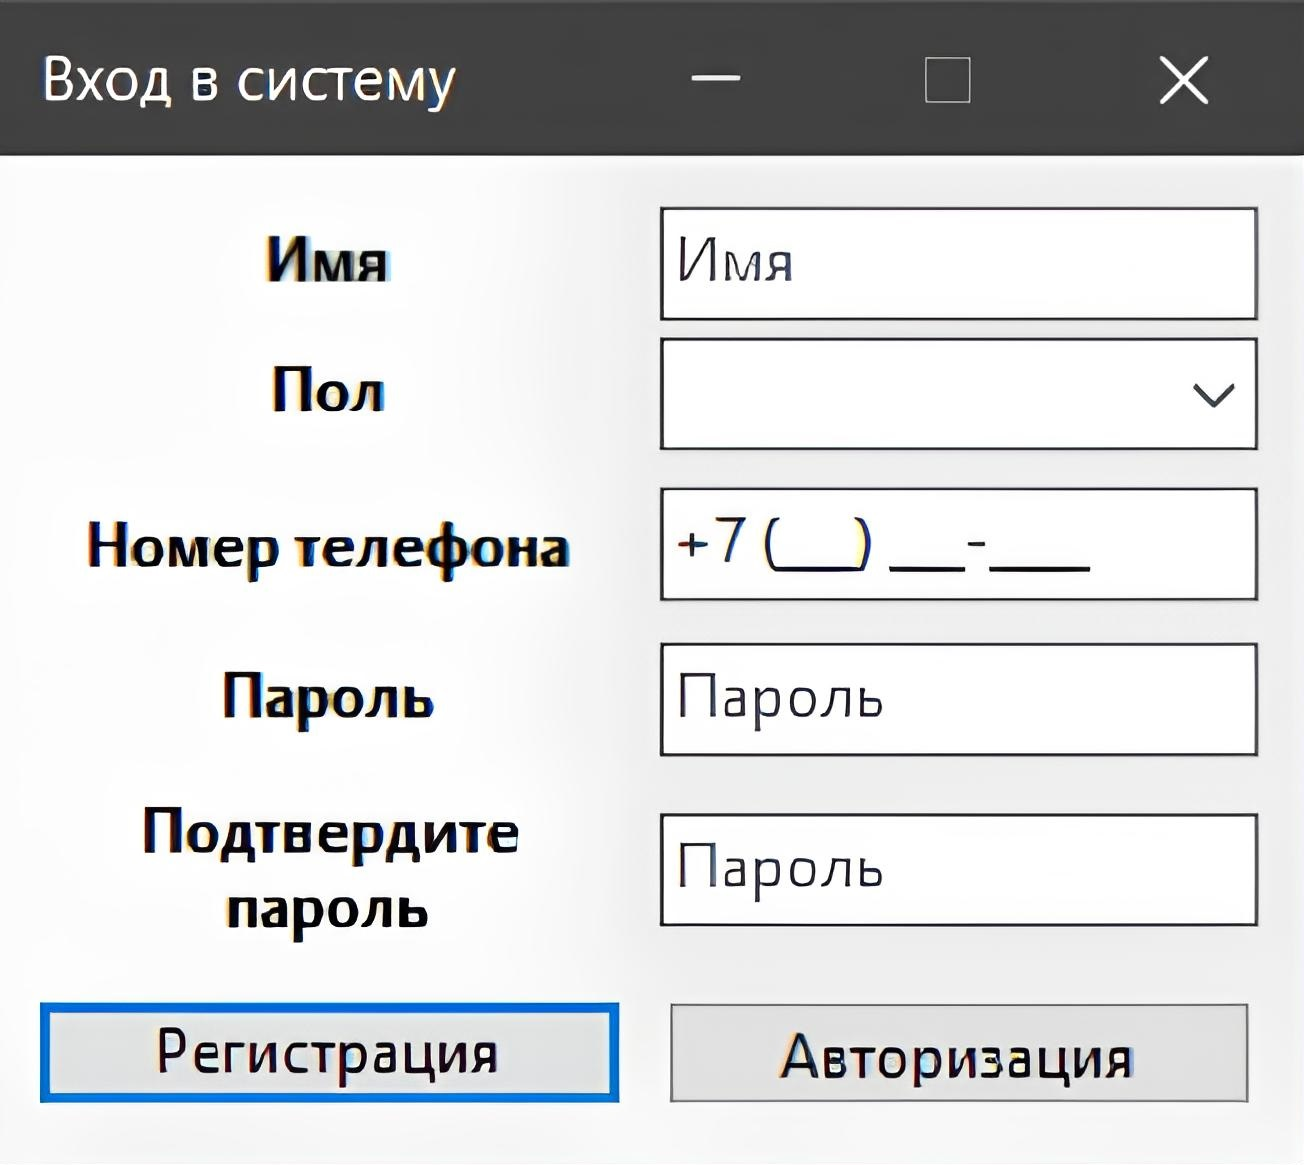
\includegraphics[width=0.4\textwidth]{images/app-enter.png}
	\caption{Интерфейс окна <<Вход в систему>>} 
	\label{fig:app-enter} 
\end{figure}

После успешного входа в систему пользователю демонстрируется главное окно приложения с панелью, содержащую вкладки <<Профиль>>, <<Мероприятия>> и <<Организация>>. 

Вкладка <<Профиль>> содержит данные о пользователе и позволяет редактировать их. Вкладка <<Мероприятия>> содержит доступные пользователю мероприятия для участия. Вкладка <<Организация>> содержит организованные пользователем мероприятия.

\begin{figure}[h!]
	\centering
	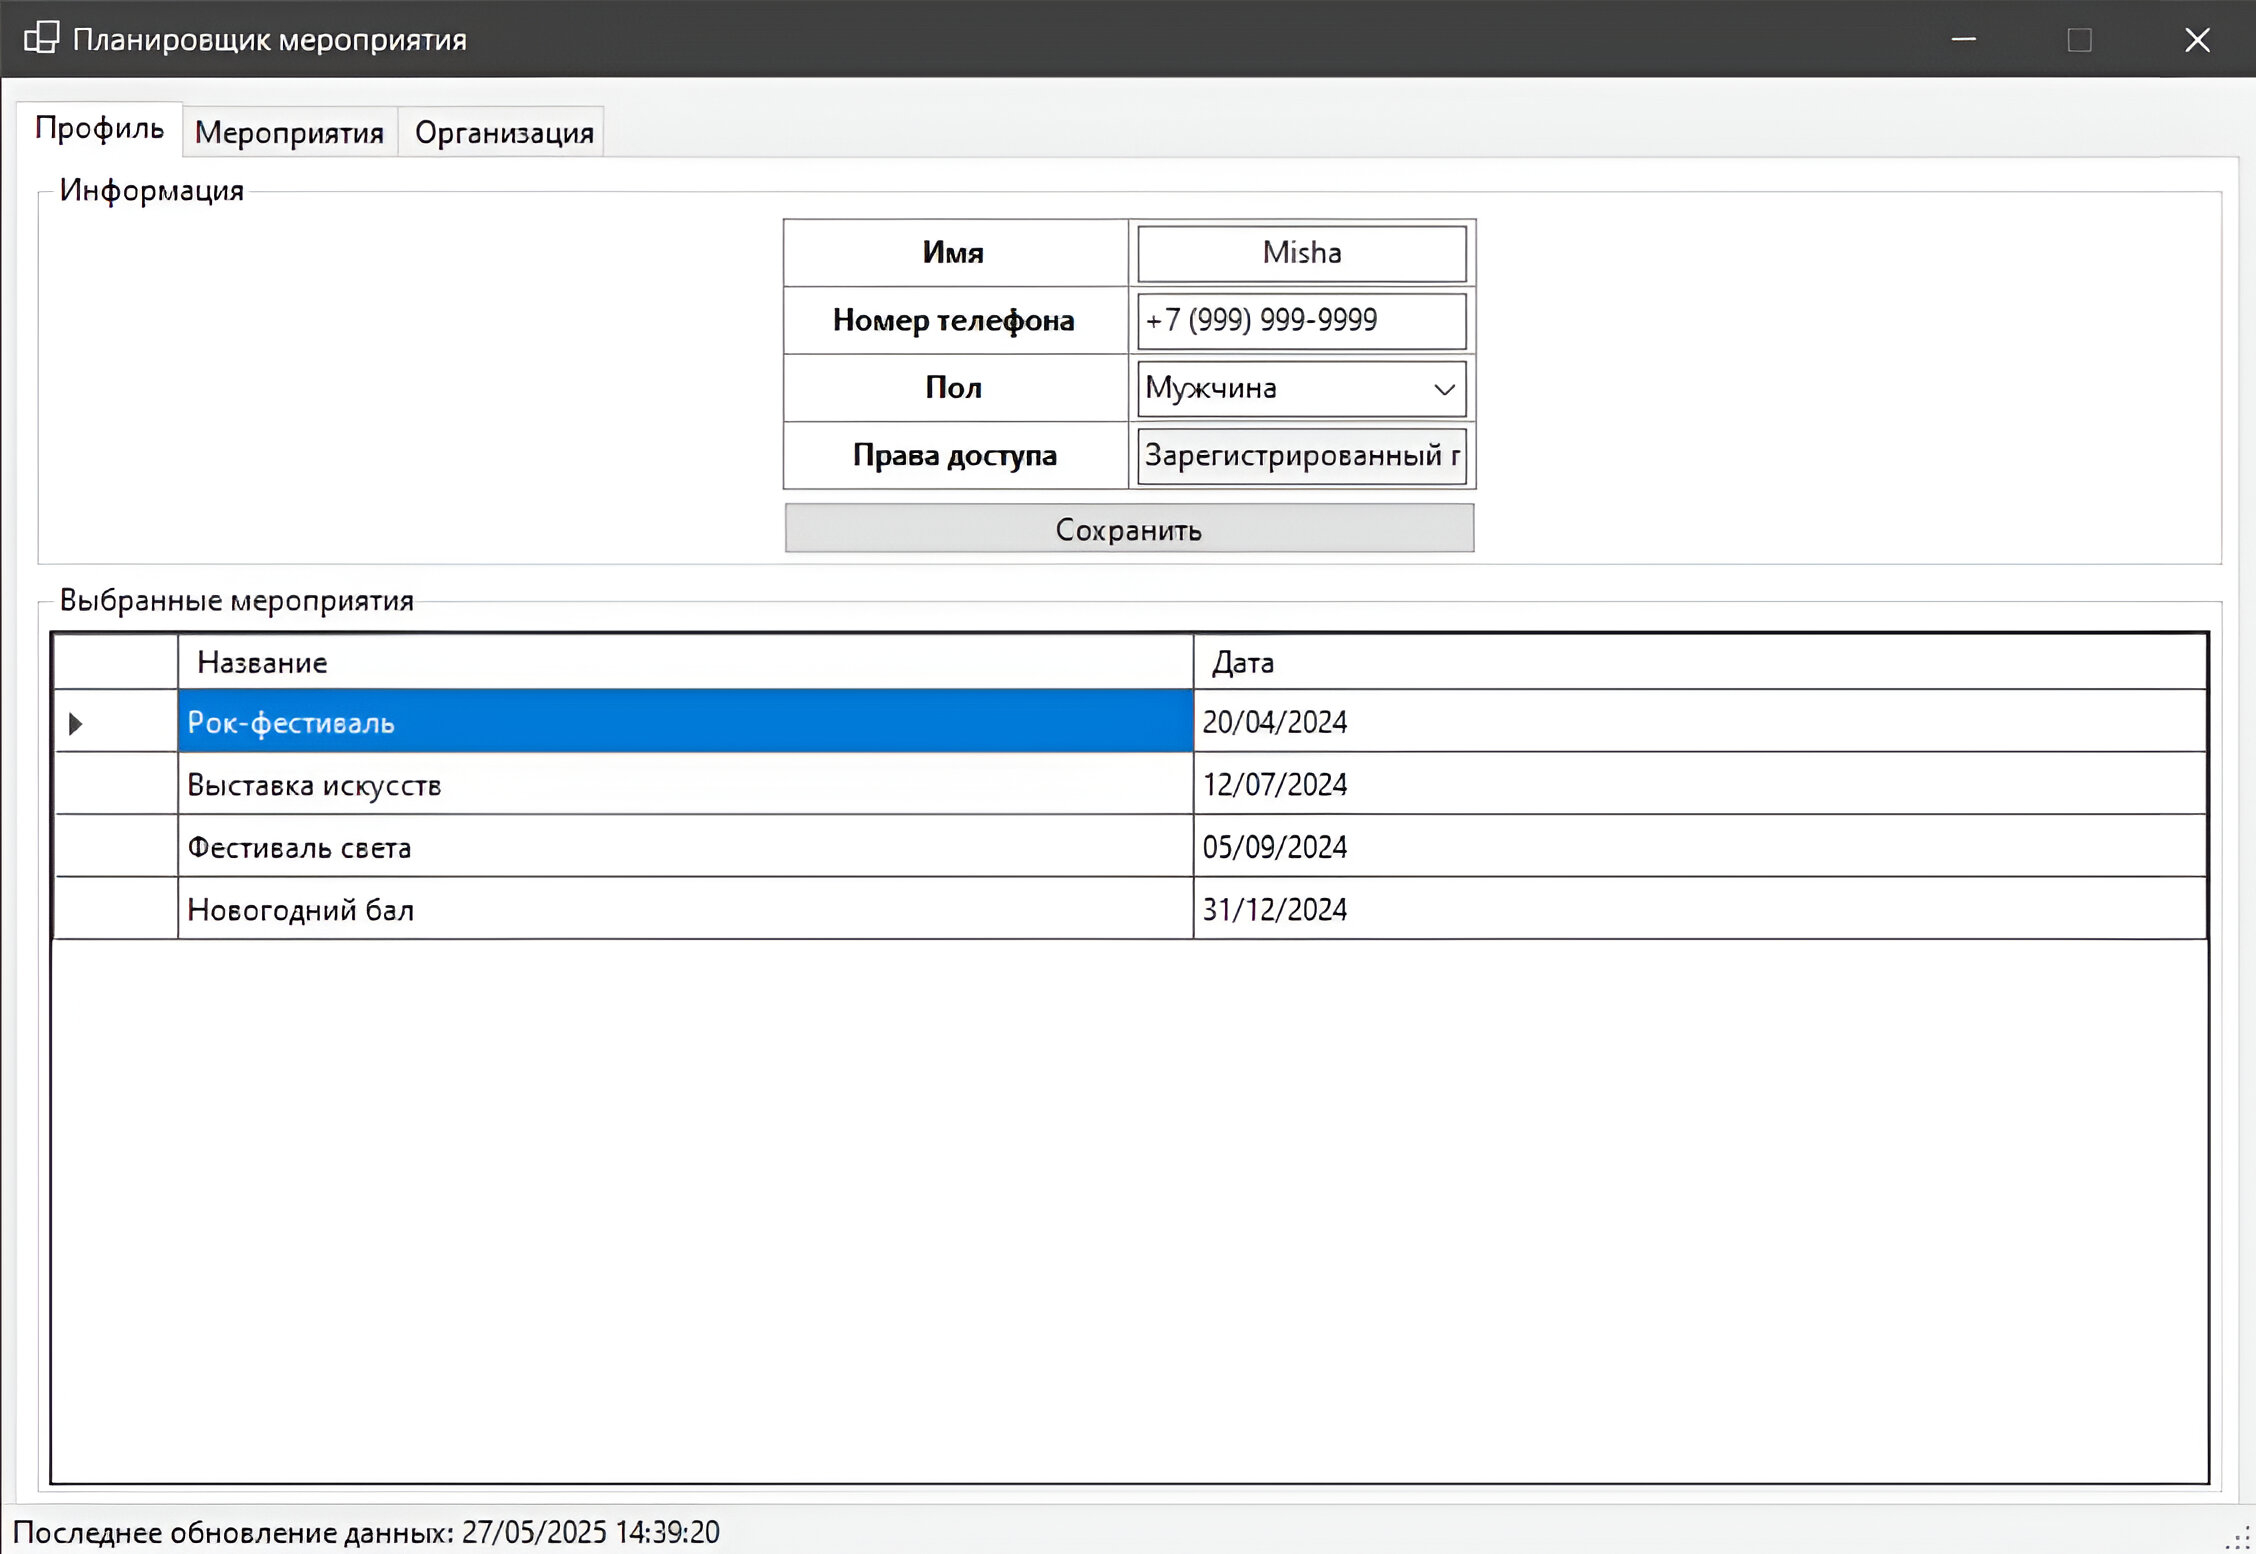
\includegraphics[width=0.93\textwidth]{images/mainwindow-1.png}
	\caption{Интерфейс главного окна приложения (часть 1)} 
	\label{fig:app-mainwindow-1} 
\end{figure}

\begin{figure}[h!]
	\centering
	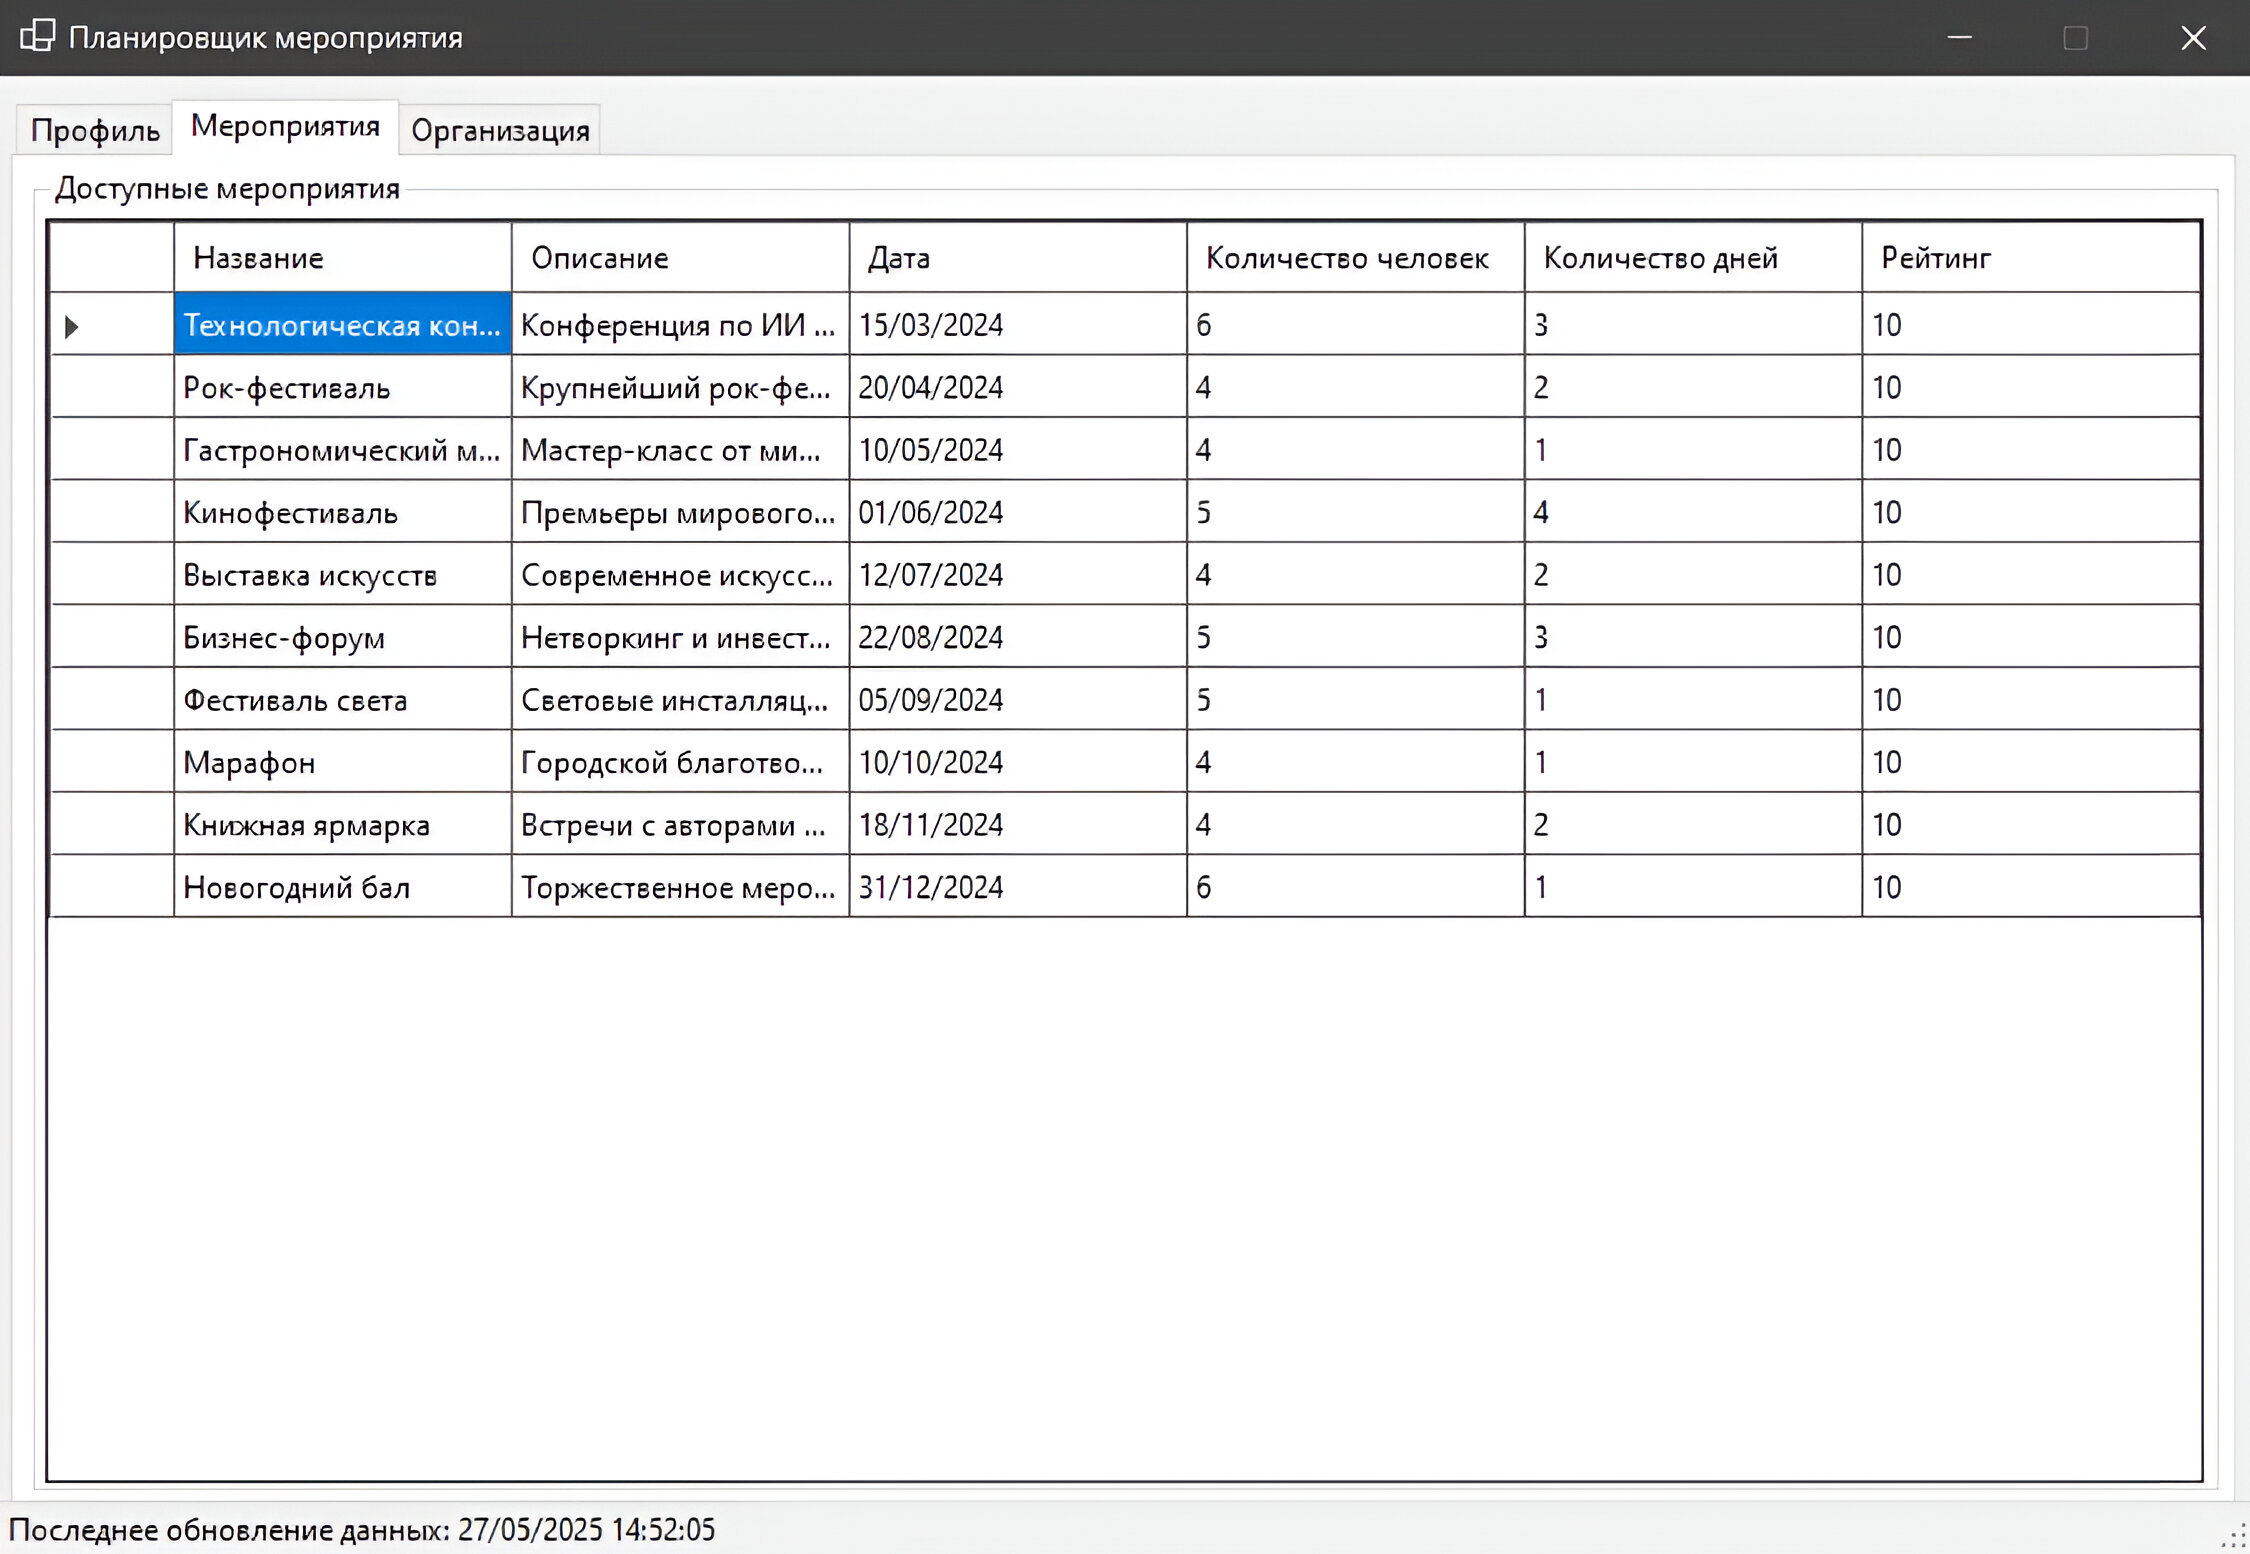
\includegraphics[width=0.93\textwidth]{images/mainwindow-2.png}
	\caption{Интерфейс главного окна приложения (часть 2)} 
	\label{fig:app-mainwindow-2} 
\end{figure}

\begin{figure}[h!]
	\centering
	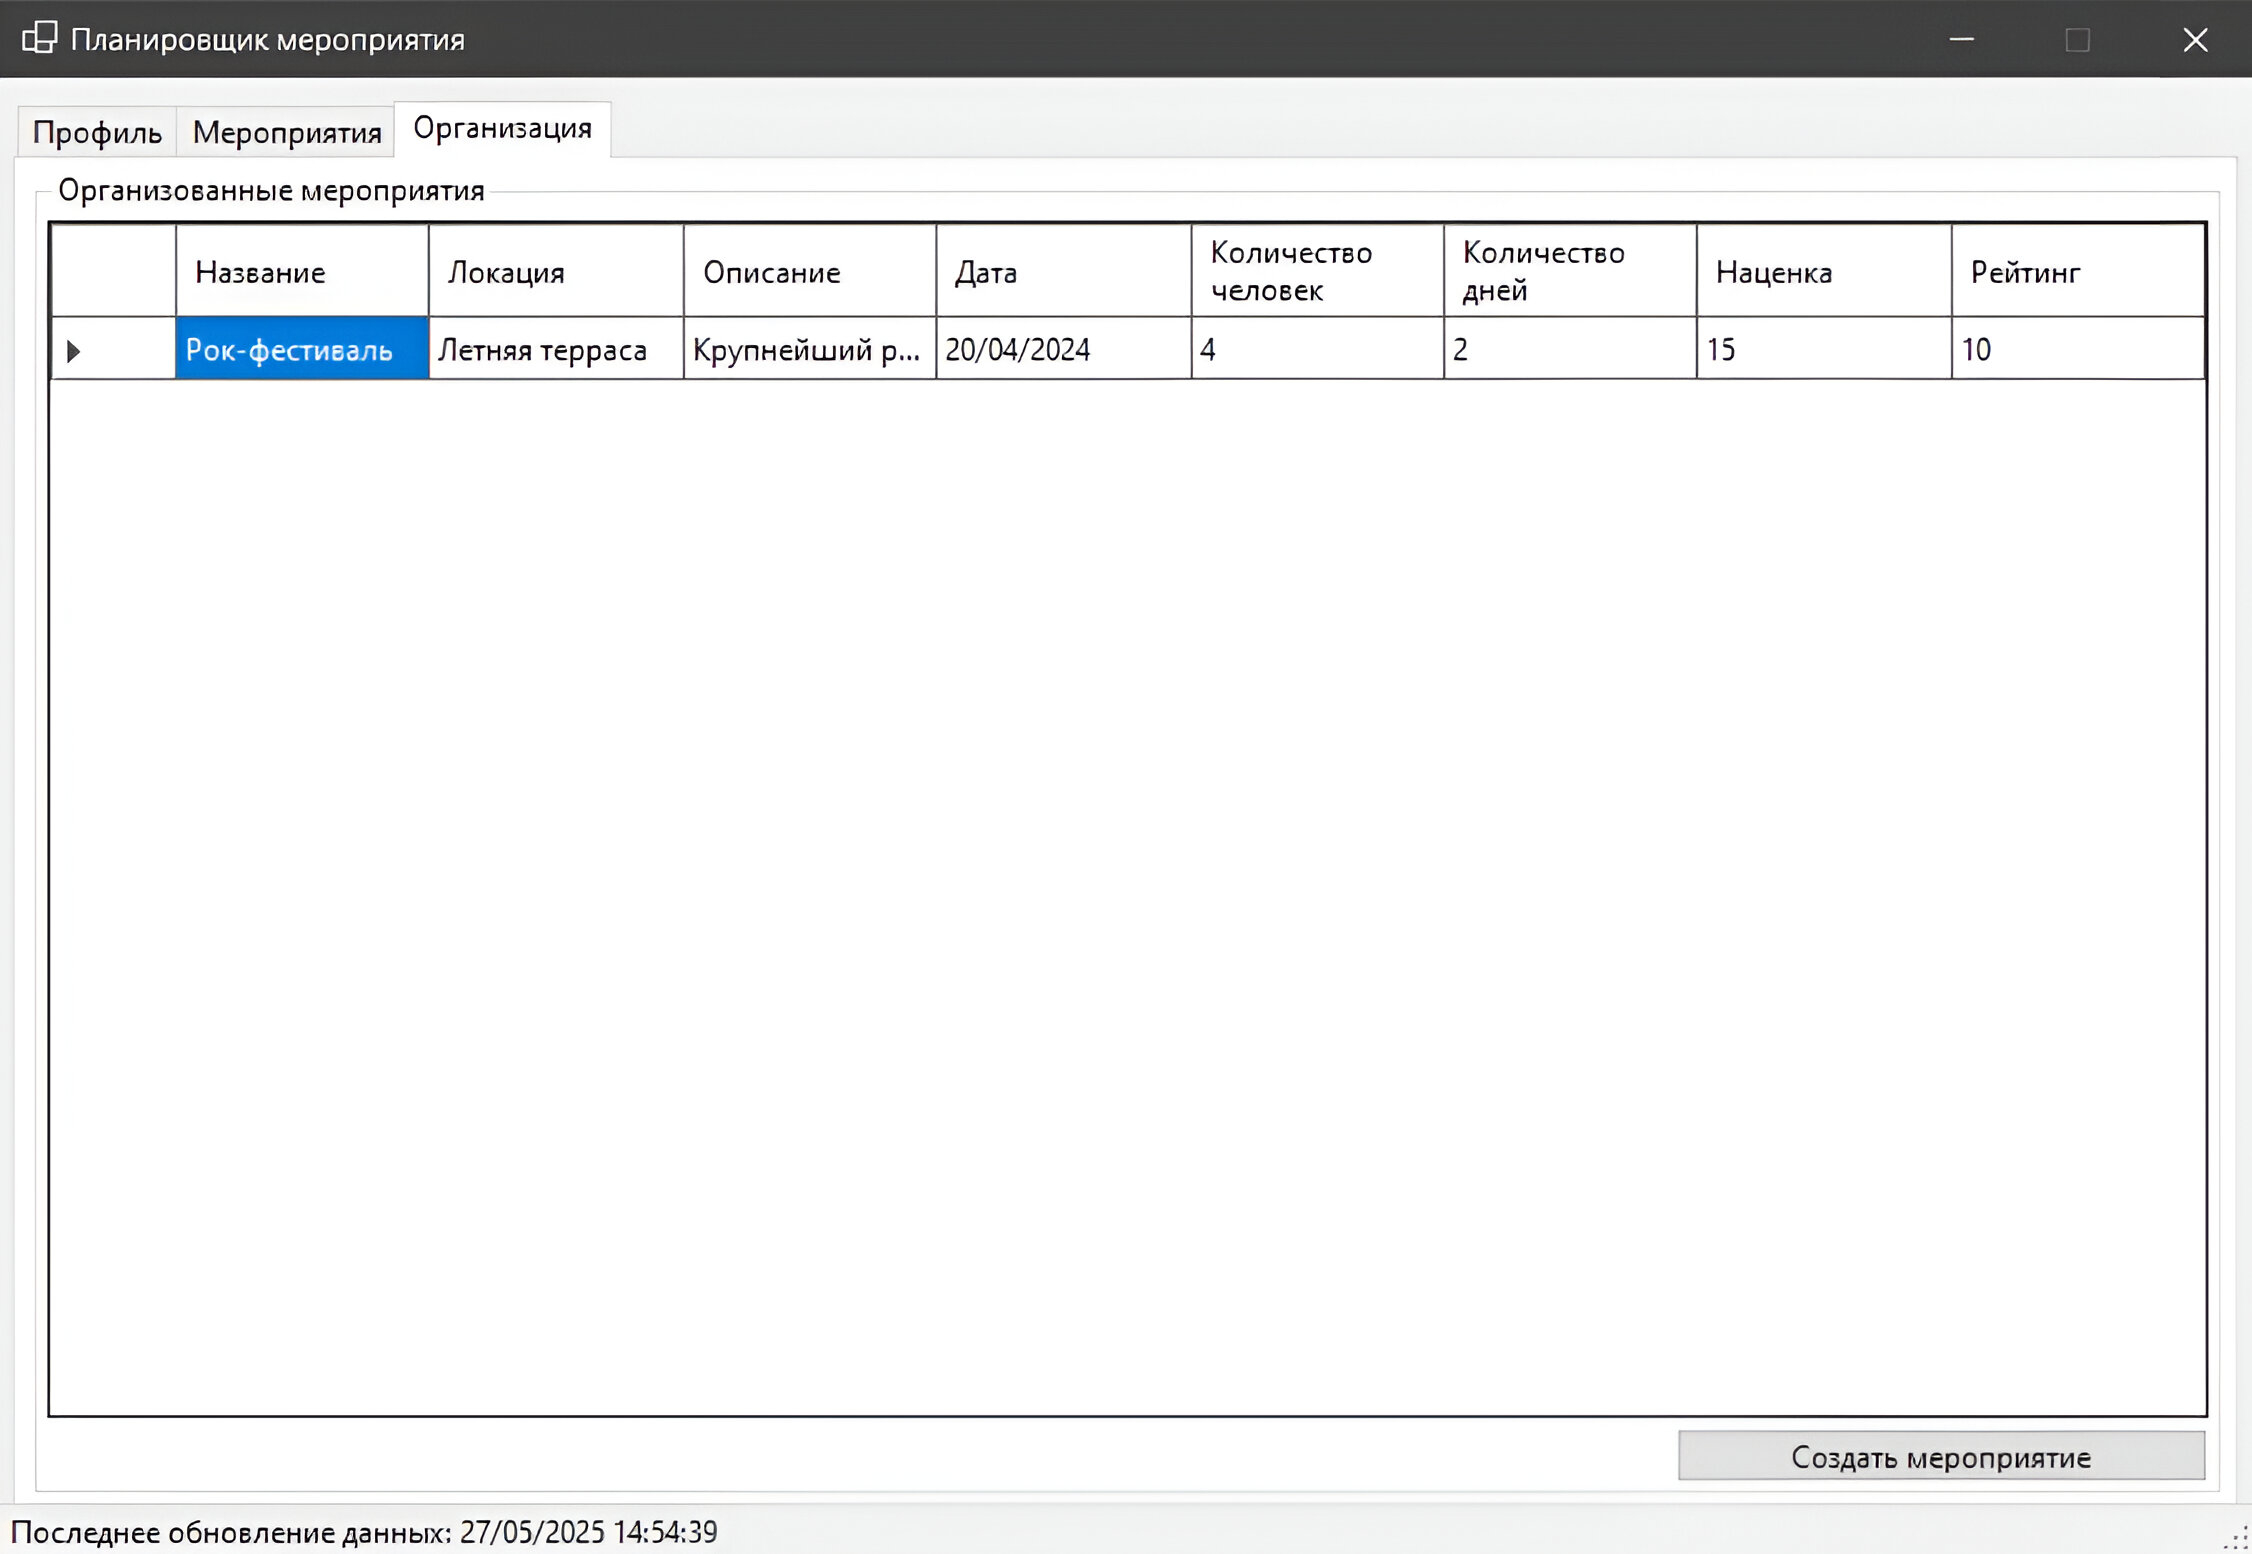
\includegraphics[width=0.93\textwidth]{images/mainwindow-3.png}
	\caption{Интерфейс главного окна приложения (часть 3)} 
	\label{fig:app-mainwindow-3} 
\end{figure}

При нажатии на данные о мероприятии, если пользователь не является администратором или организатором мероприятия, ему демонстрируется окно <<Информация о мероприятии>>, содержащее информацию о связанном мероприятии и позволяющее взаимодействовать с ней.

\begin{figure}[h!]
	\centering
	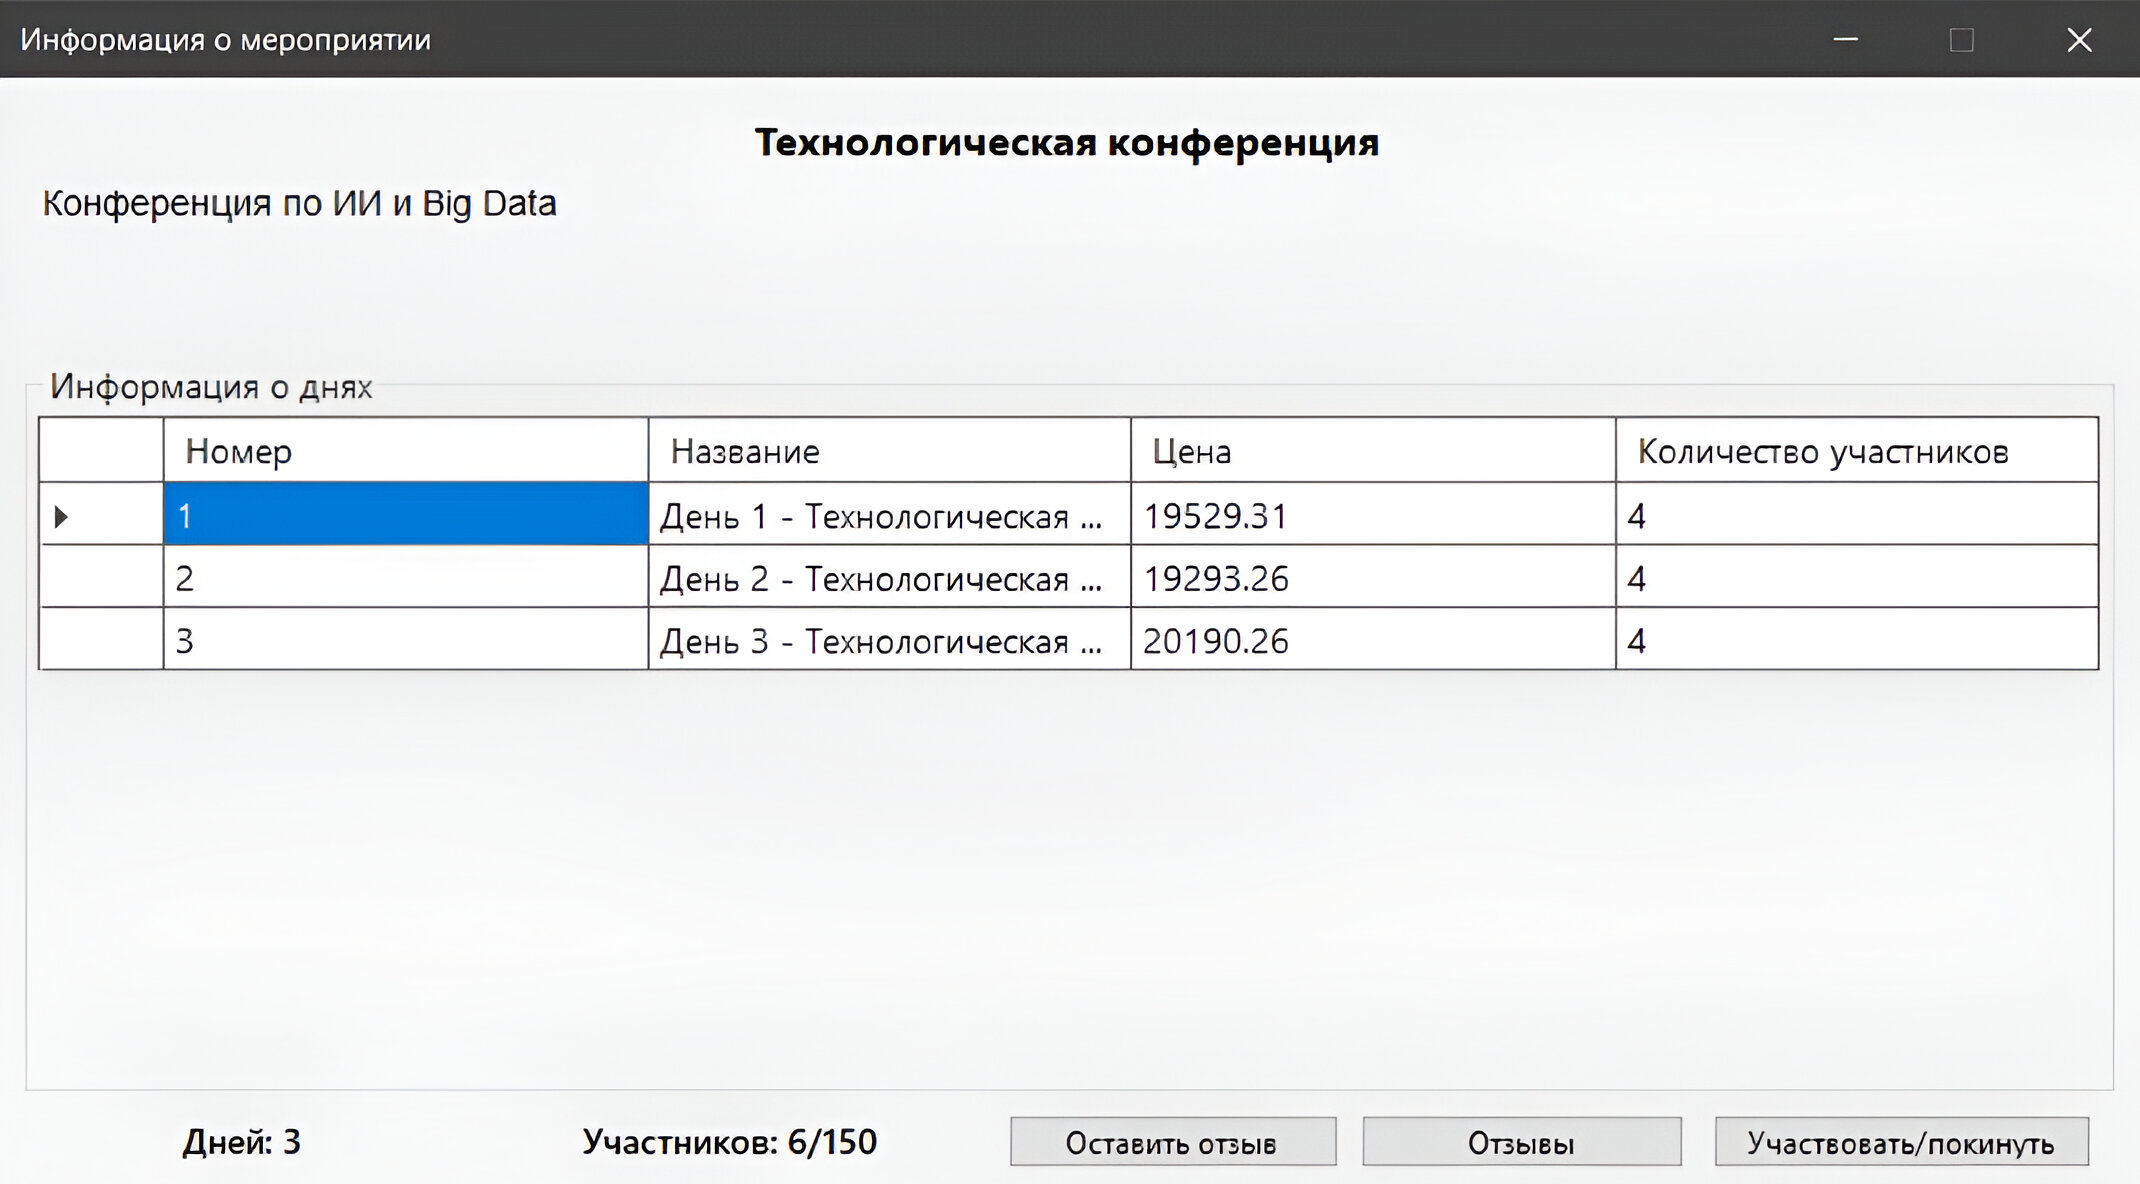
\includegraphics[width=1\textwidth]{images/app-event-info.png}
	\caption{Интерфейс окна <<Информация о мероприятии>>} 
	\label{fig:app-event-info} 
\end{figure}

При нажатии на текстовое поле содержащее количество участников мероприятия пользователю демонстрируется окно <<Участники меропрития>>, содержащую список участников мероприятия.
\begin{figure}[h!]
	\centering
	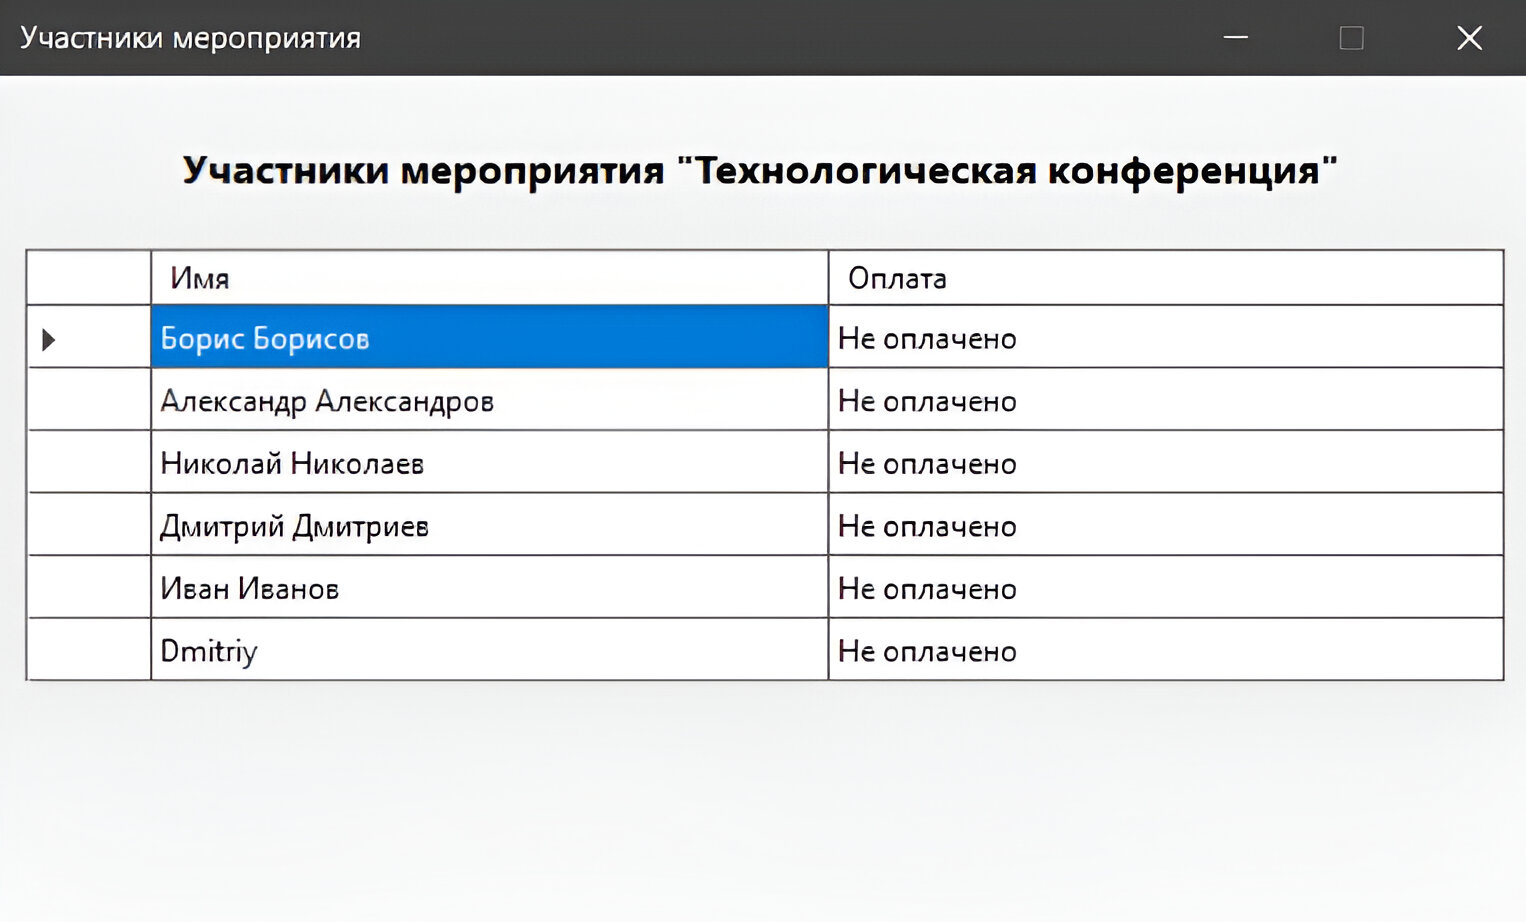
\includegraphics[width=0.7\textwidth]{images/app-event-persons.png}
	\caption{Интерфейс окна <<Участники мероприятия>>} 
	\label{fig:app-event-persons} 
\end{figure}

При нажатии на кнопку <<Оставить отзыв>> пользователю демонстрируется окно <<Отзыв>>, позволяющее создать отзыв о мероприятии.
\begin{figure}[h!]
	\centering
	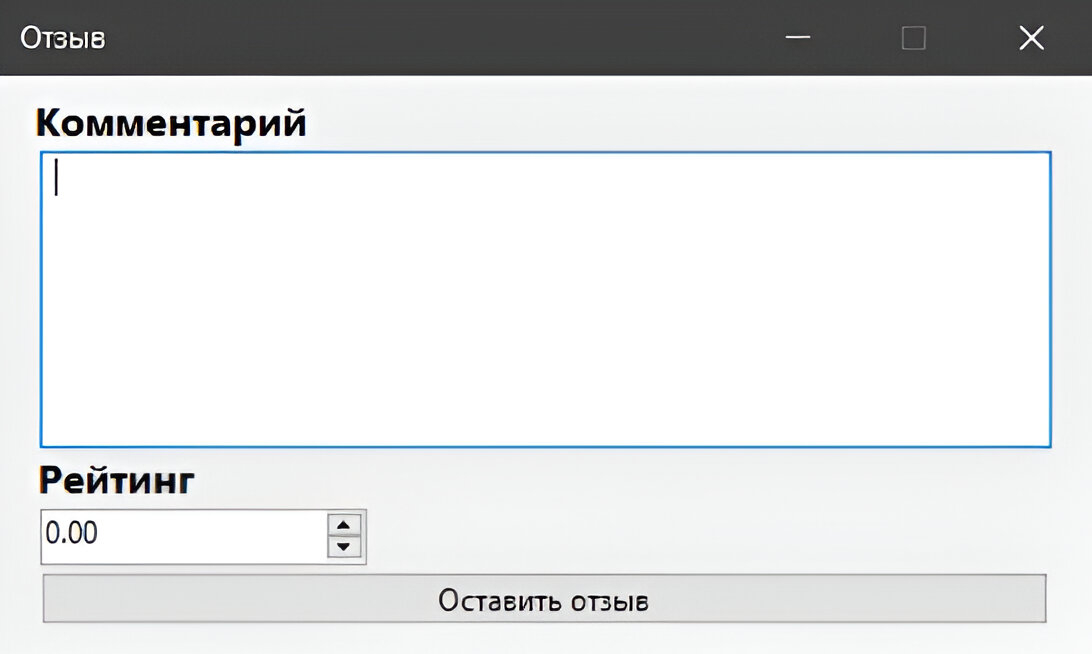
\includegraphics[width=0.7\textwidth]{images/app-event-feedback.png}
	\caption{Интерфейс окна <<Отзыв>>} 
	\label{fig:app-event-feedback} 
\end{figure}

При нажатии на кнопку <<Отзывы>> пользователю демонстрируется окно <<Отзывы мероприятия>>, содержащее список всех отзывов мероприятия.
\begin{figure}[h!]
	\centering
	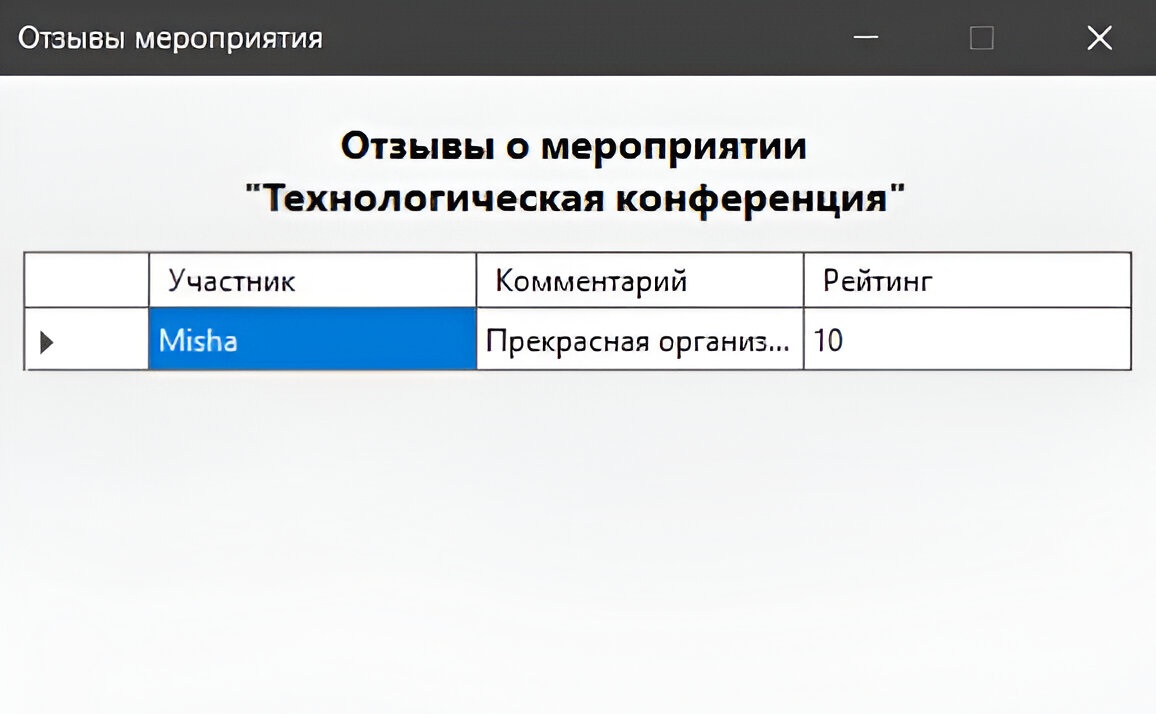
\includegraphics[width=0.7\textwidth]{images/app-event-feedbacks.png}
	\caption{Интерфейс окна <<Отзывы мероприятия>>} 
	\label{fig:app-event-feedbacks} 
\end{figure}

\newpage

При нажатии на кнопку <<Участвовать/покинуть>> пользователю демонстрируется окно <<Дни присутствия>>, позволяющее участвовать в мероприятии, покинуть его или изменить дни присутствия.

\begin{figure}[h!]
	\centering
	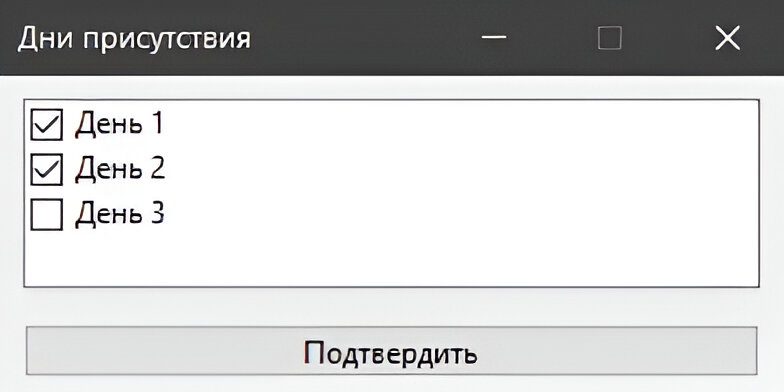
\includegraphics[width=0.7\textwidth]{images/app-event-participation.png}
	\caption{Интерфейс окна <<Дни присутствия>>} 
	\label{fig:app-event-participation} 
\end{figure}

При нажатии на данные о дне мероприятия пользователю демонстрируется окно <<Информация о дне мероприятия>>, содержащее всю информацию о связанном дне мероприятия.
\begin{figure}[h!]
	\centering
	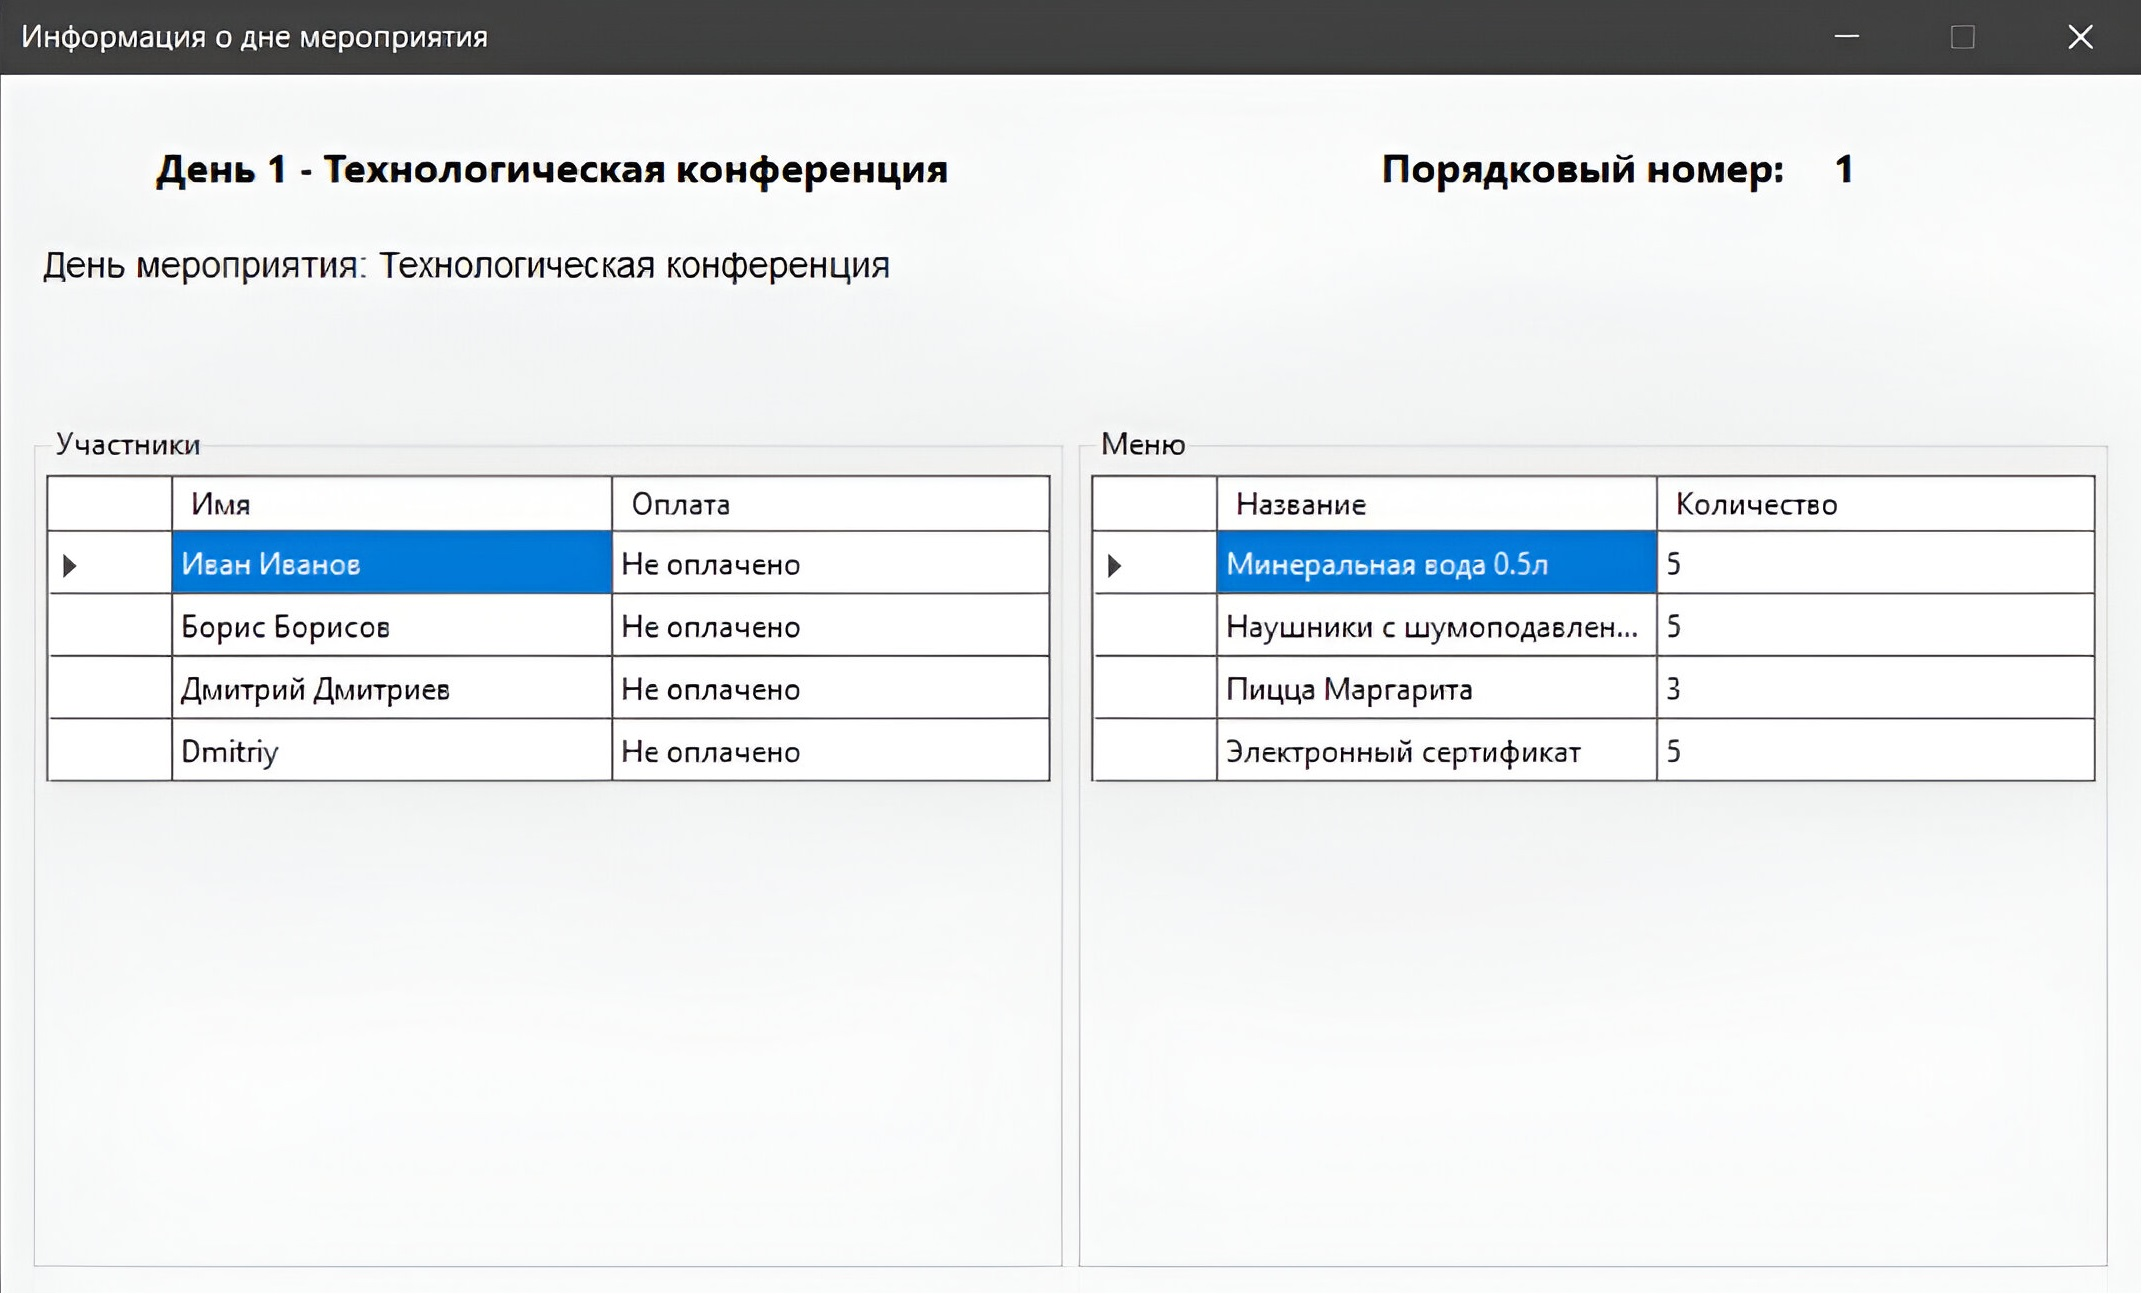
\includegraphics[width=1\textwidth]{images/app-day-info.png}
	\caption{Интерфейс окна <<Информация о дне мероприятия>>} 
	\label{fig:app-day-info} 
\end{figure}

\newpage

При нажатии на данные о мероприятии, если пользователь является администратором или организатором мероприятия, ему демонстрируется окно <<Организация мероприятия>>, содержащее всю информацию о связанном мероприятии и позволяющее взаимодействовать с ней.
\begin{figure}[h!]
	\centering
	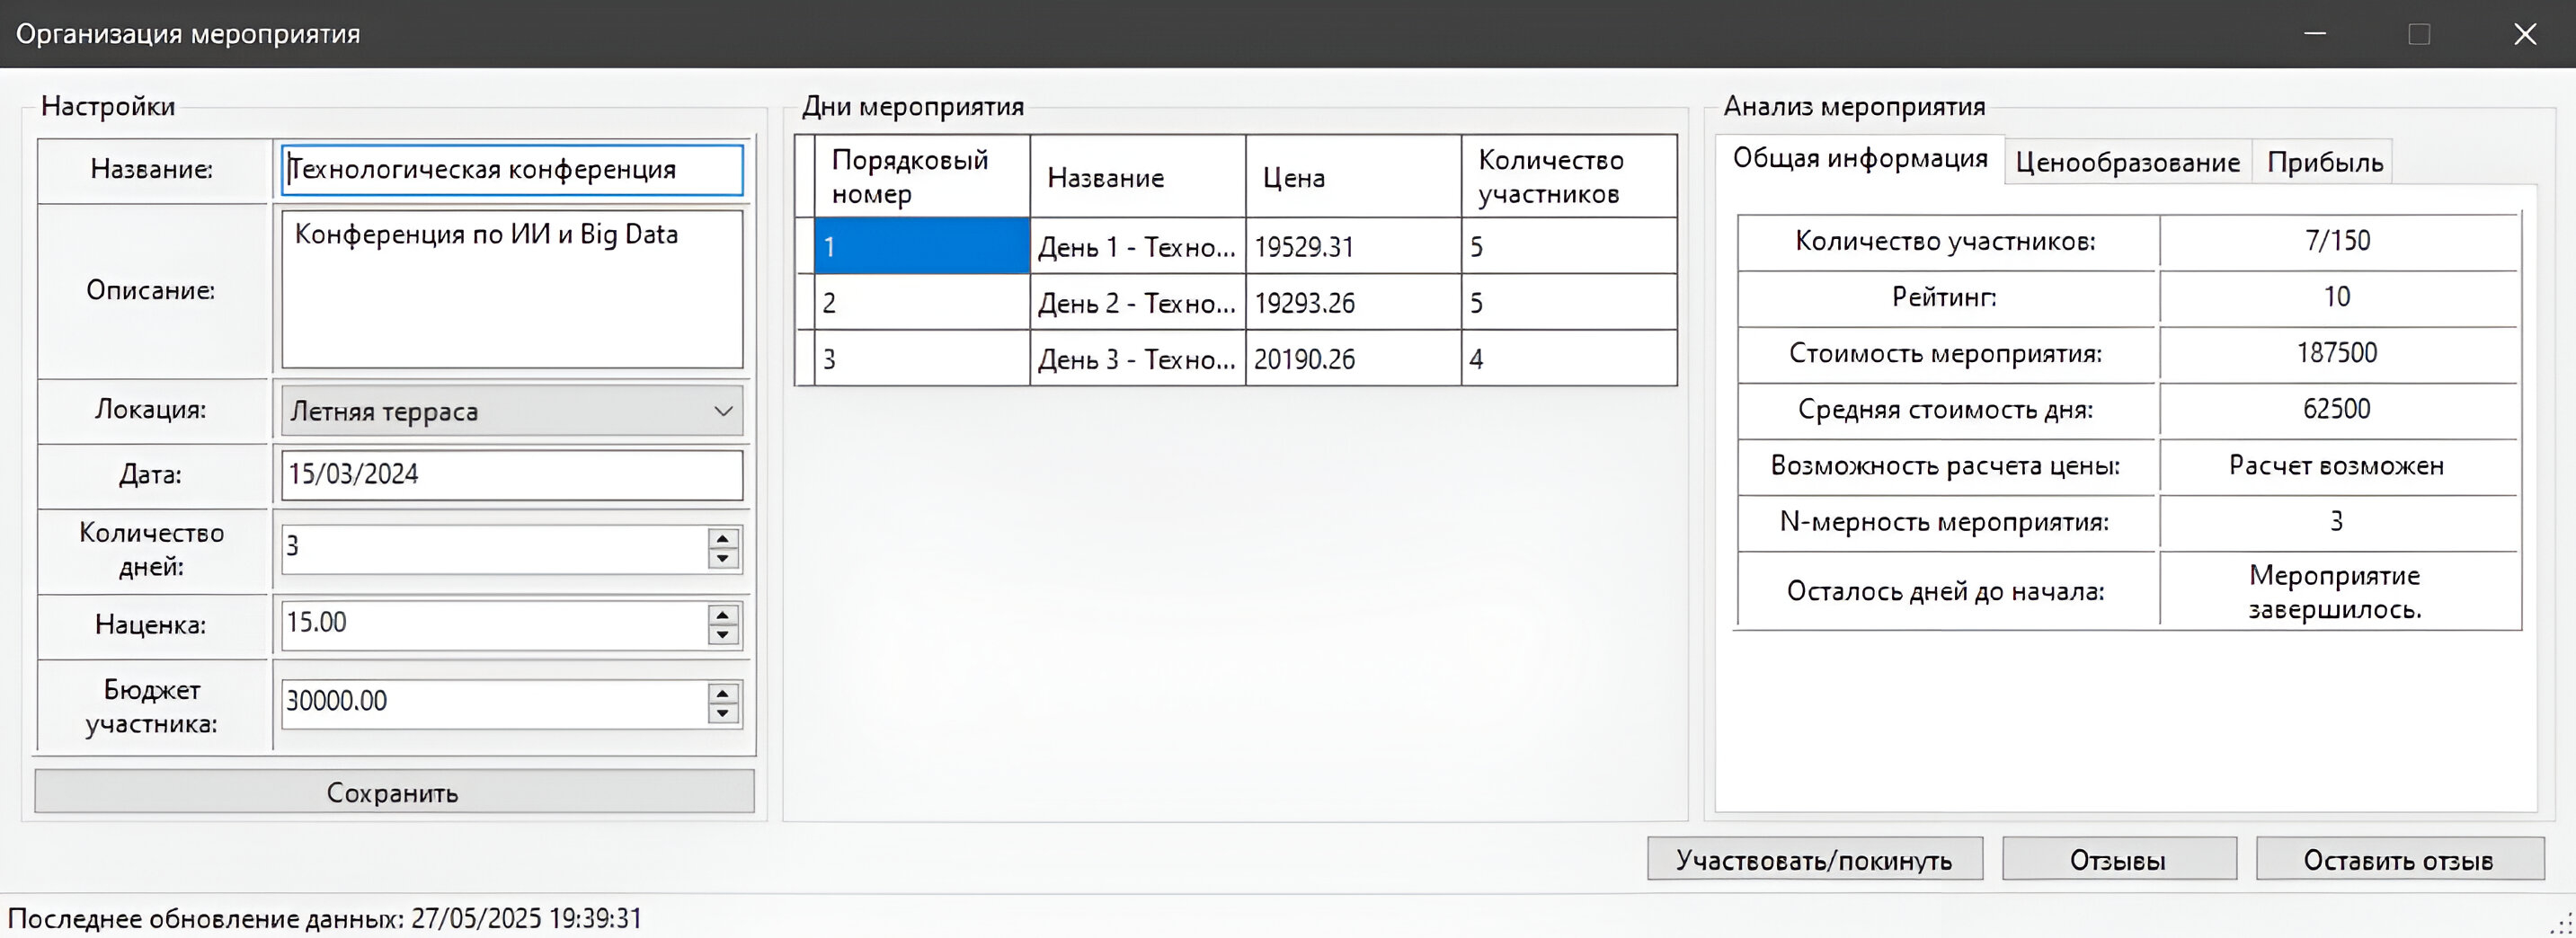
\includegraphics[width=1\textwidth]{images/app-event-organization.png}
	\caption{Интерфейс окна <<Организация мероприятия>>} 
	\label{fig:app-event-organization} 
\end{figure}
\begin{figure}[h!]
	\centering
	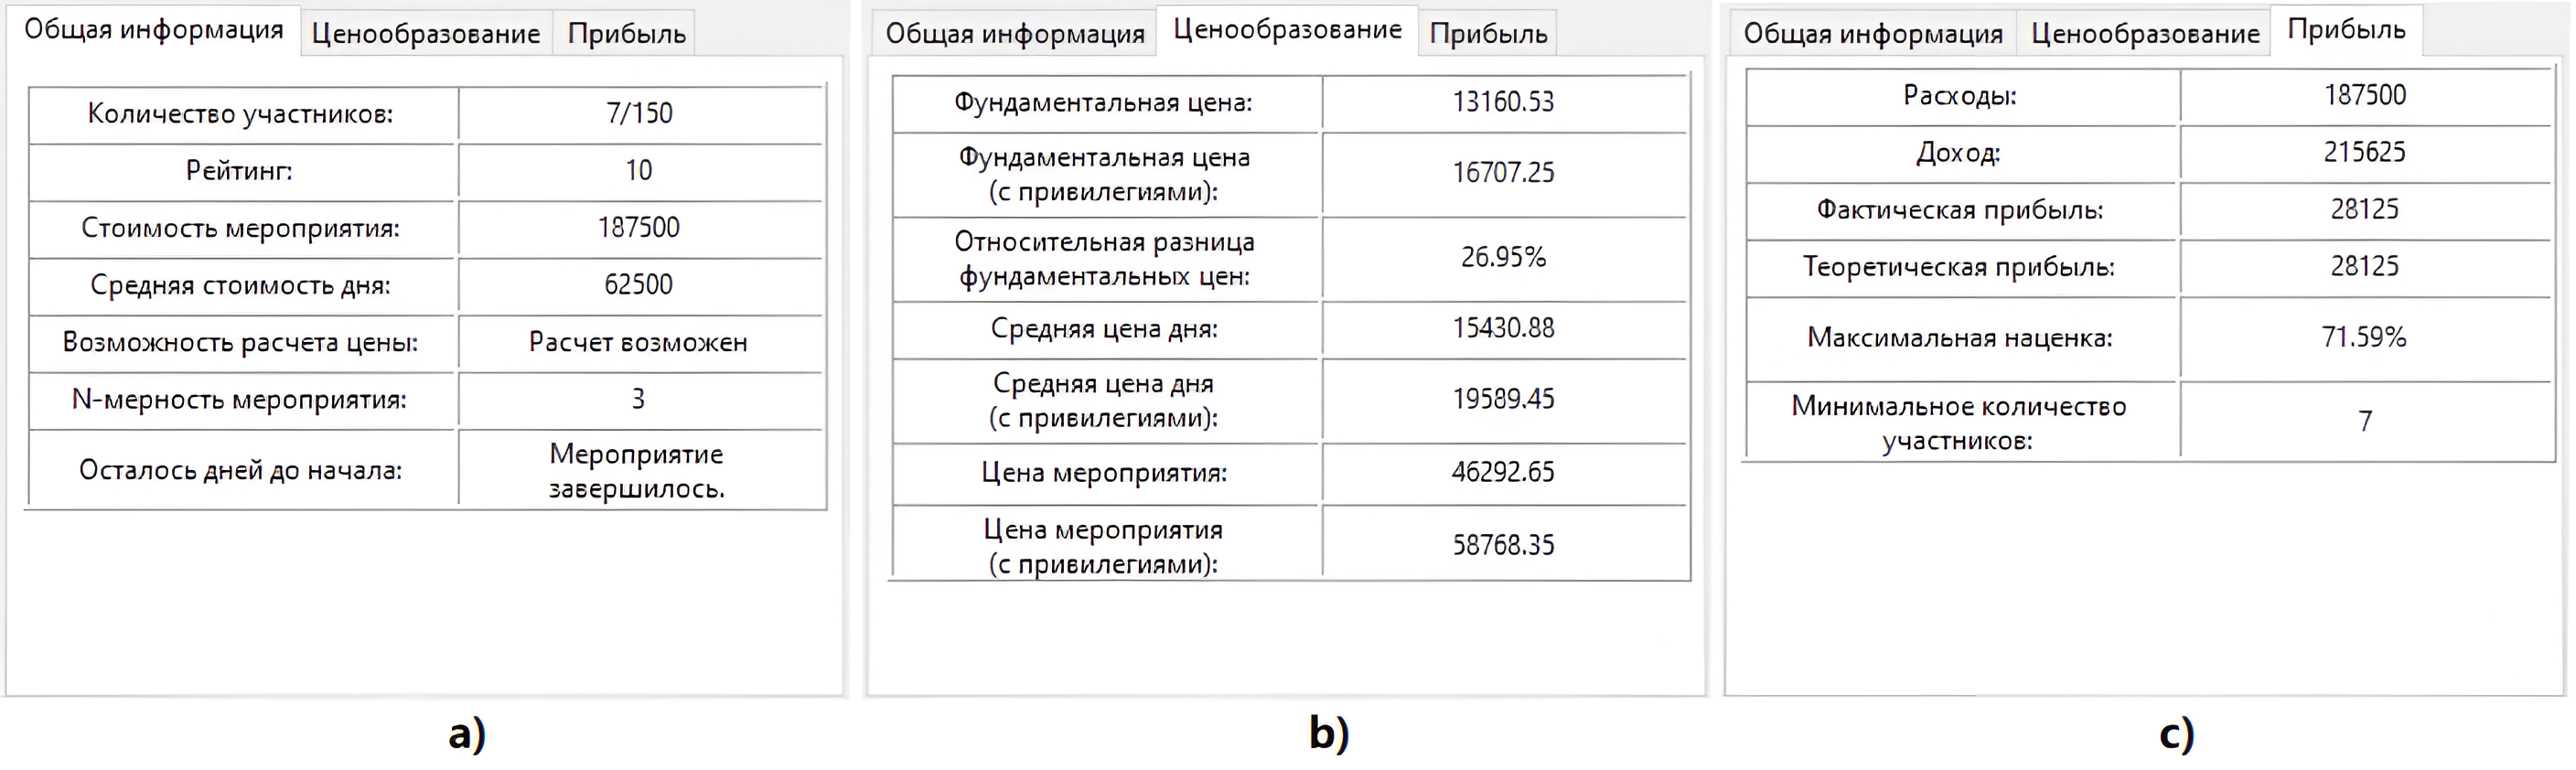
\includegraphics[width=1\textwidth]{images/app-event-analyze.png}
	\caption{Вкладки панели в группе <<Анализ мероприятия>>: общая информация (a), ценообразование (b), прибыль (c)} 
	\label{fig:app-event-analyze} 
\end{figure}

\newpage

При нажатии на данные о дне мероприятия пользователю демонстрируется окно <<Организация дня мероприятия>>, содержащее всю информацию о связанном дне мероприятия и позволяющее взаимодействовать с ней.

\begin{figure}[h!]
	\centering
	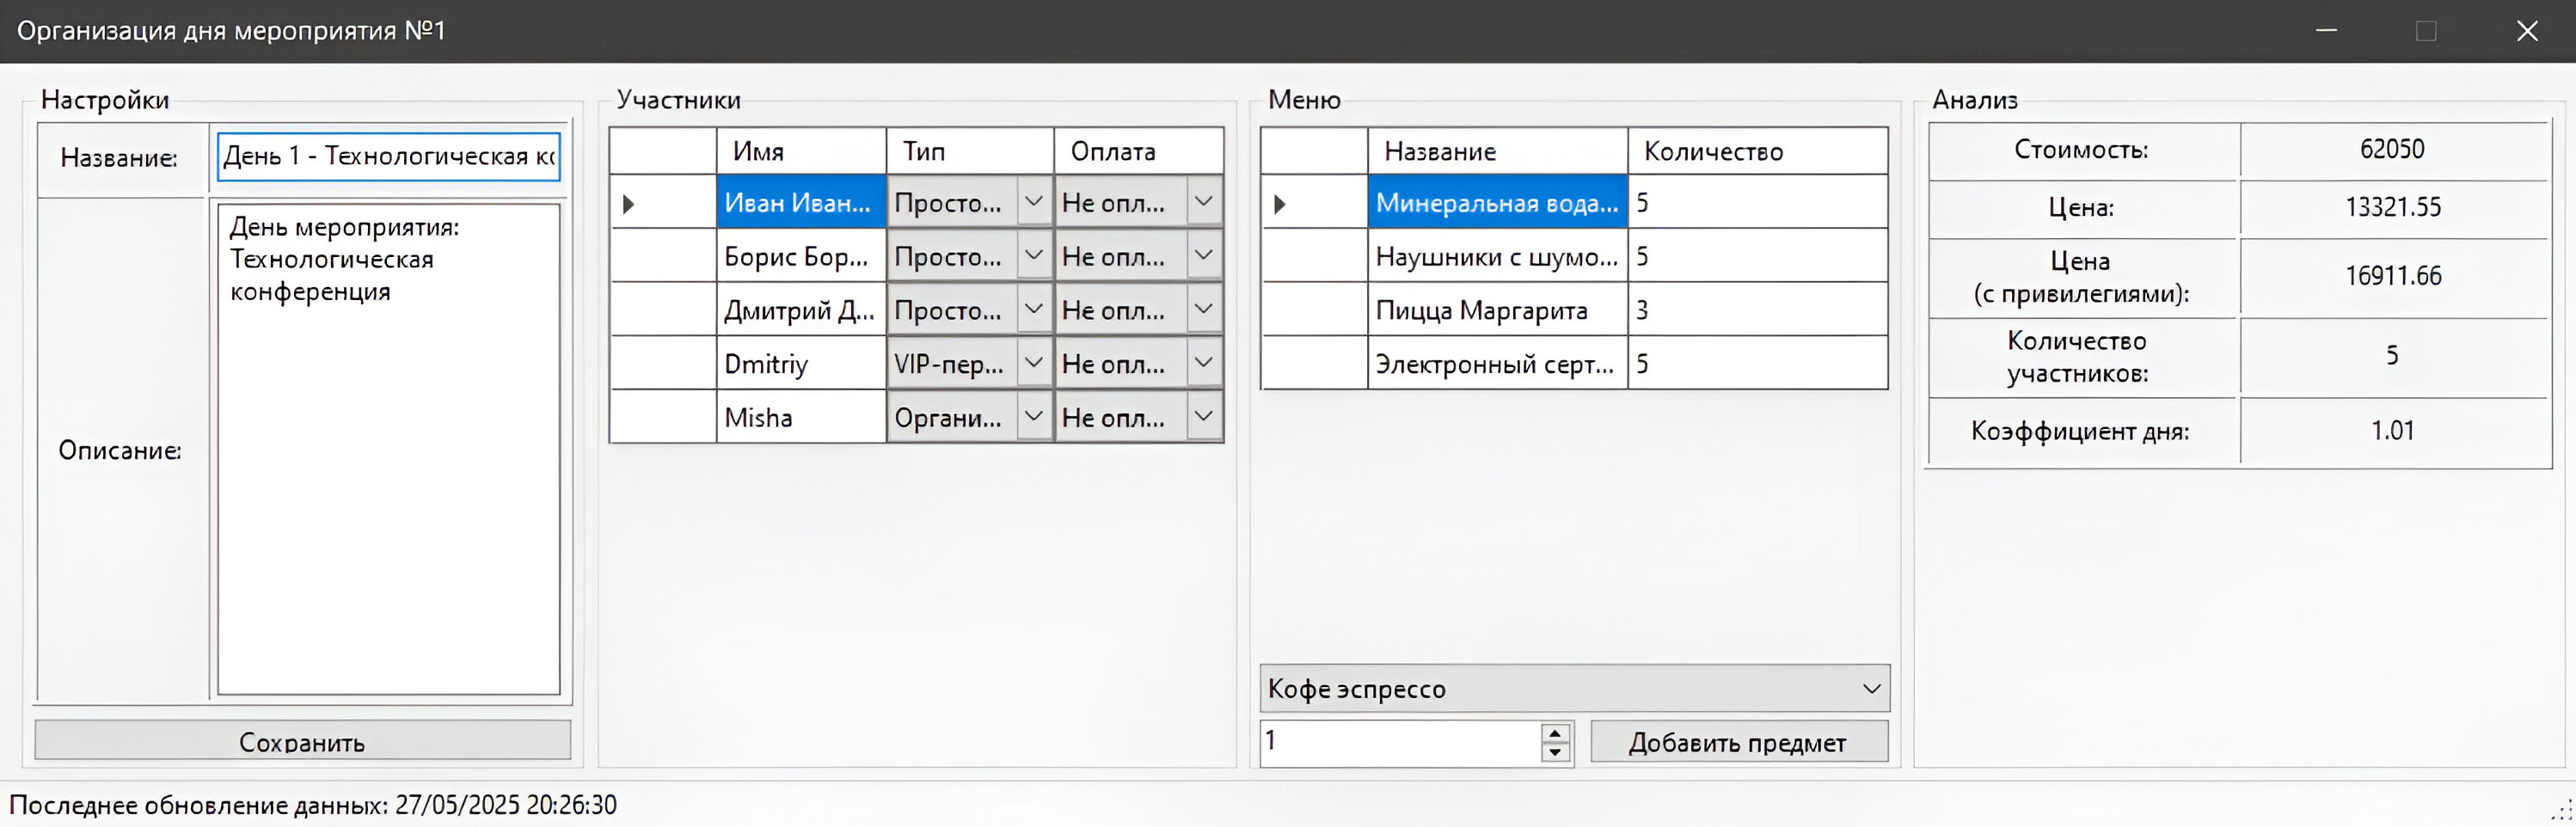
\includegraphics[width=1\textwidth]{images/app-day-organization.png}
	\caption{Интерфейс окна <<Организация дня мероприятия>>} 
	\label{fig:app-day-organization} 
\end{figure}

\section{Тестирование}

Классы эквивалентности для входа в систему представлены в таблицах~\ref{tbl:name-classes},~\ref{tbl:gender-classes},~\ref{tbl:phone-classes}~и~\ref{tbl:password-classes}.

\begin{table}[h]
	\centering
	\caption{Классы эквивалентности для поля <<Имя>>}
	\label{tbl:name-classes}
	\begin{tabularx}{\textwidth}{|X|X|X|}
		\hline
		\textbf{Класс} & \textbf{Примеры} & \textbf{Ожидаемый результат} \\
		\hline
		Непустая строка & Иван, Anna-Maria, 123 & Успешная проверка \\
		\hline
		Пустая строка & Пустое поле & Ошибка: «Имя обязательно» \\
		\hline
	\end{tabularx}
\end{table}

\begin{table}[h]
	\centering
	\caption{Классы эквивалентности для поля <<Пол>>}
	\label{tbl:gender-classes}
	\begin{tabularx}{\textwidth}{|X|X|X|}
		\hline
		\textbf{Класс} & \textbf{Примеры} & \textbf{Ожидаемый результат} \\
		\hline
		Корректный пол & Мужской, женский & Успешная проверка \\
		\hline
		Пустое значение & Не выбран пол & Ошибка: «Пол обязателен» \\
		\hline
	\end{tabularx}
\end{table}

\begin{table}[h]
	\centering
	\caption{Классы эквивалентности для поля <<Номер телефона>>}
	\label{tbl:phone-classes}
	\begin{tabularx}{\textwidth}{|X|X|X|}
		\hline
		\textbf{Класс} & \textbf{Примеры} & \textbf{Ожидаемый результат} \\
		\hline
		Корректный формат & +7 (999) 123-45-67 & Успешная проверка формата \\
		\hline
		Некорректный формат & +7 (999) 123, пустая строка & Ошибка: «Некорректный номер» \\
		\hline
		Занятый номер & +7 (919) 345-56-7 & Ошибка: «Номер занят» \\
		\hline
		Несуществующий номер & +7 (919) 345-56-79 & Ошибка: «Пользователь не найден» \\
		\hline
		Уже зарегистрированный номер & Использовать существующий в базе данных номер & Успешная авторизация \\
		\hline
	\end{tabularx}
\end{table}

\newpage

\begin{table}[h]
	\centering
	\caption{Классы эквивалентности для поля <<Пароль>>}
	\label{tbl:password-classes}
	\begin{tabularx}{\textwidth}{|X|X|X|}
		\hline
		\textbf{Класс} & \textbf{Примеры} & \textbf{Ожидаемый результат} \\
		\hline
		Верный пароль & Password123 & Успешная авторизация \\
		\hline
		Пустой пароль & Пустая строка & Ошибка: «Пароль обязателен» \\
		\hline
		Неверный пароль & WrongPassword & Ошибка: «Неверный пароль» \\
		\hline
	\end{tabularx}
\end{table}

Все проведенные тесты были успешно пройдены.

\section{Вывод}

В технологической части работы были представлены выборы системы управления базами данных и средств реализации приложения, описаны структуры приложения и базы данных с сопоставлением типов данных, интерфейс пользователя, а также исходный код программы и базы данных.

\clearpage
